\chapter{Representation of vortex variability in climate models}
\label{cha:models}


 \begin{figure}
 \centering
 \noindent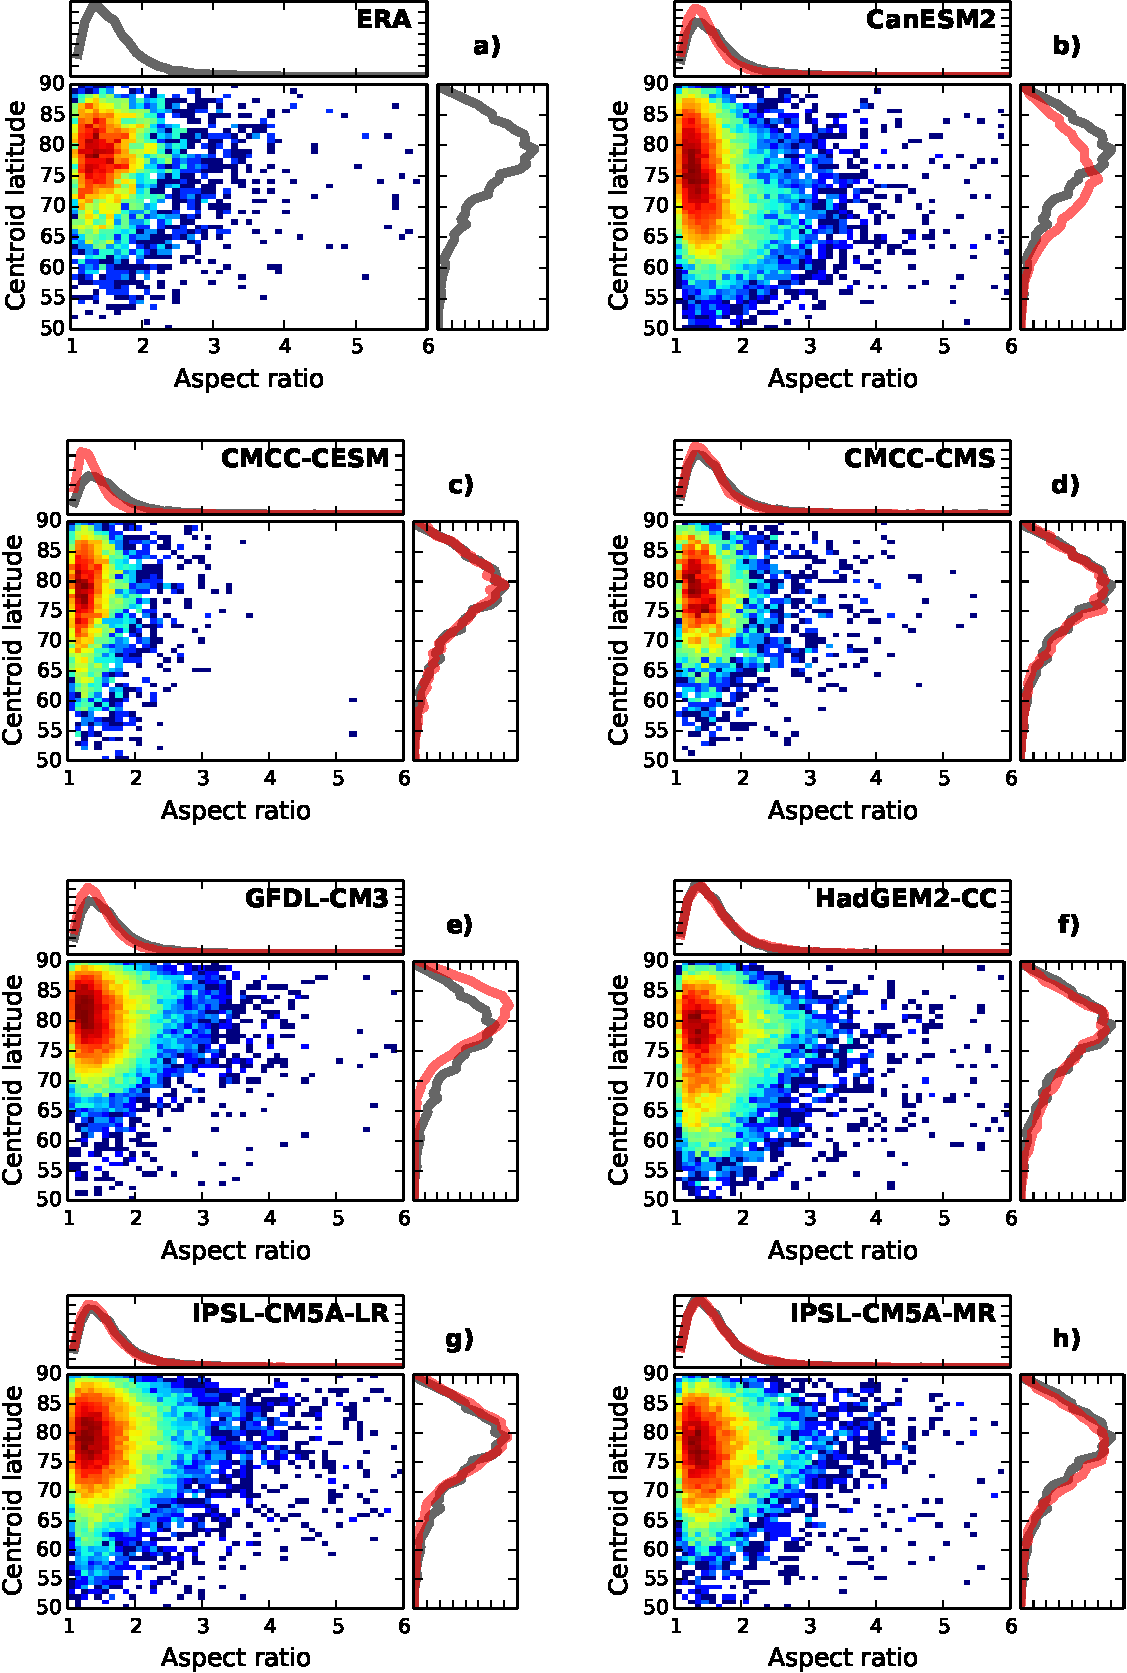
\includegraphics[width=\textwidth]{figures/chapter-models/moments_stats1.pdf}
 \caption[]{}
 \label{Fig2}
 \end{figure}

 \begin{figure}
 \ContinuedFloat
 \centering
 \noindent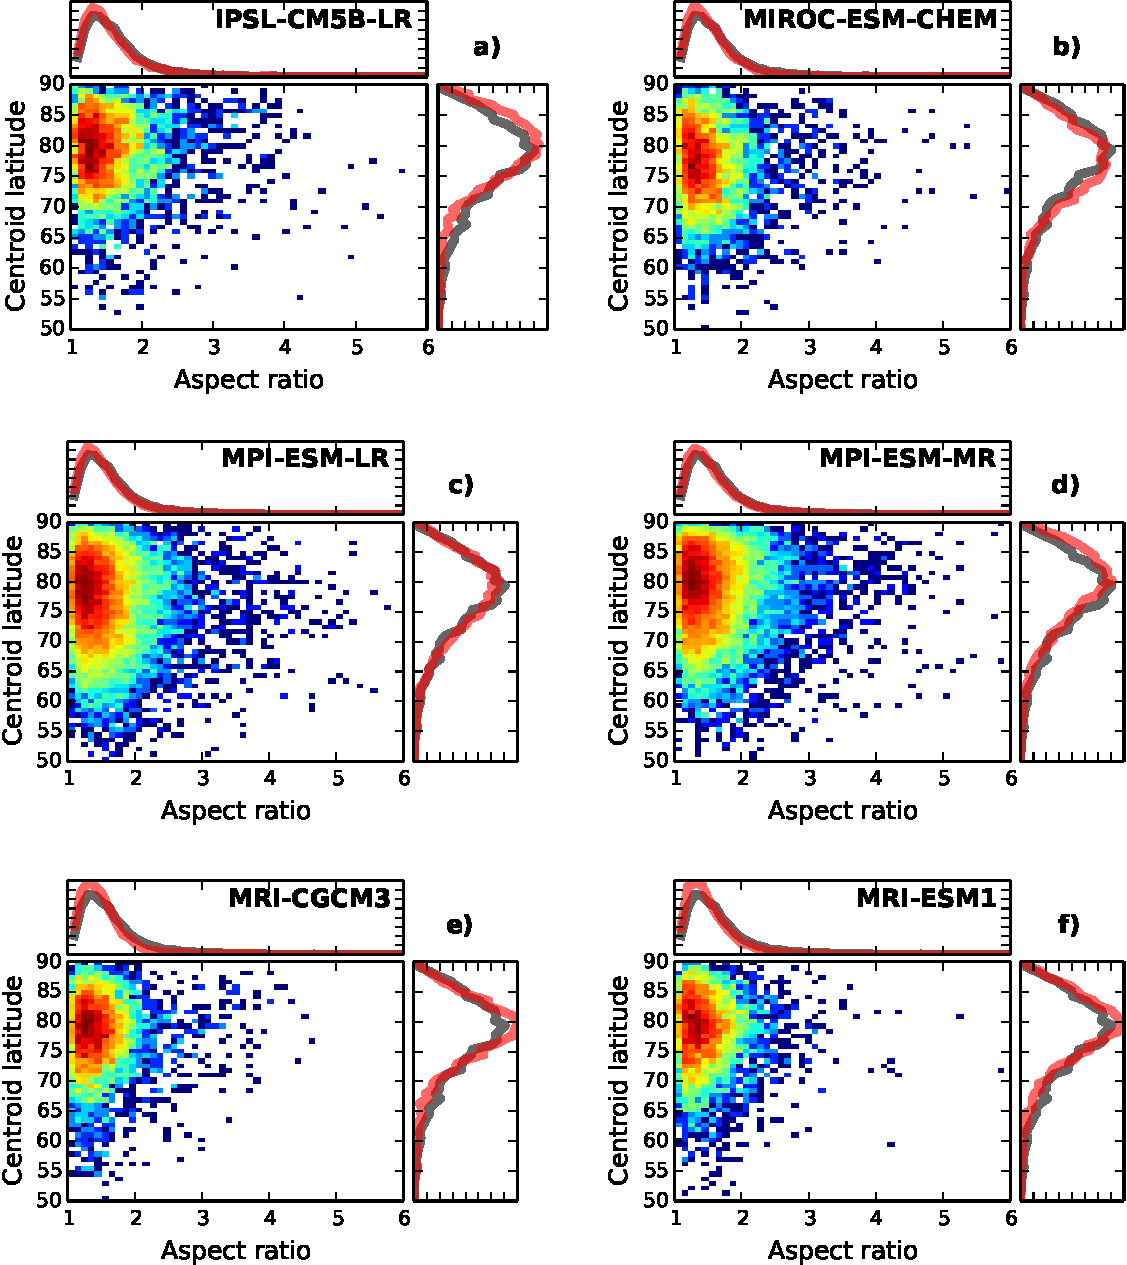
\includegraphics[width=\textwidth]{figures/chapter-models/moments_stats2.pdf}
 \caption[]{(Continued)}
 \label{Fig2}
 \end{figure}
 
\begin{figure}
 \centering
 \noindent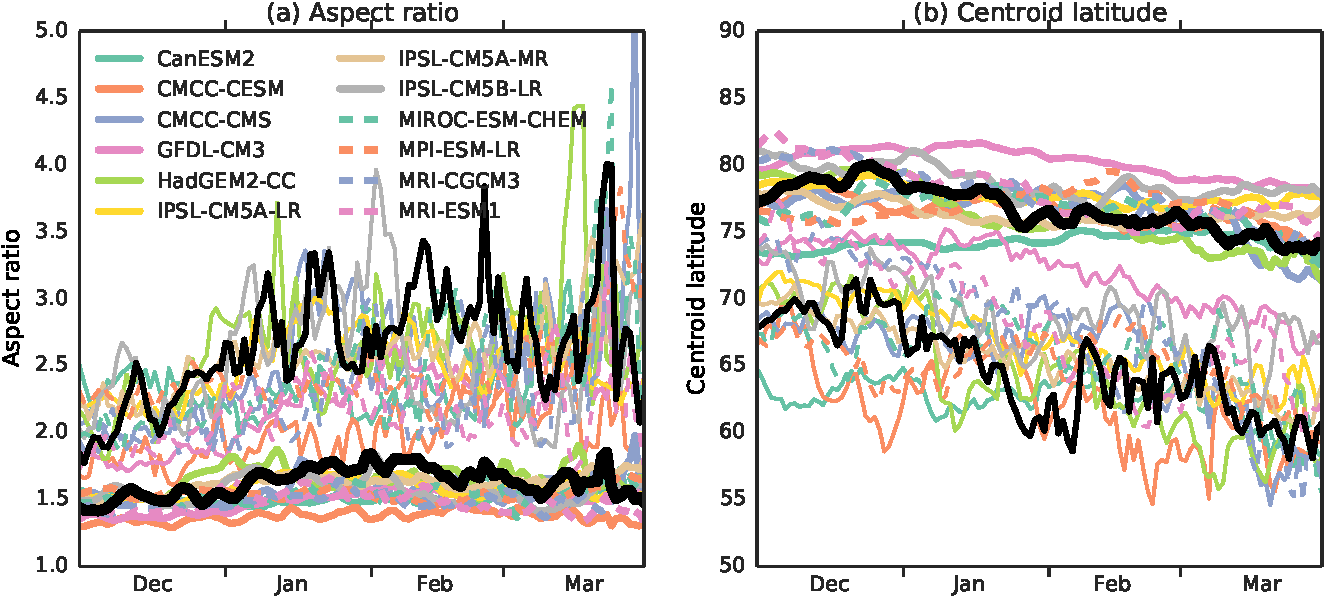
\includegraphics[width=\textwidth]{figures/chapter-models/moments_seasonal_stats.pdf}
 \caption[]{}
 \label{Fig2}
 \end{figure}




 \begin{figure}
 \centering
 \noindent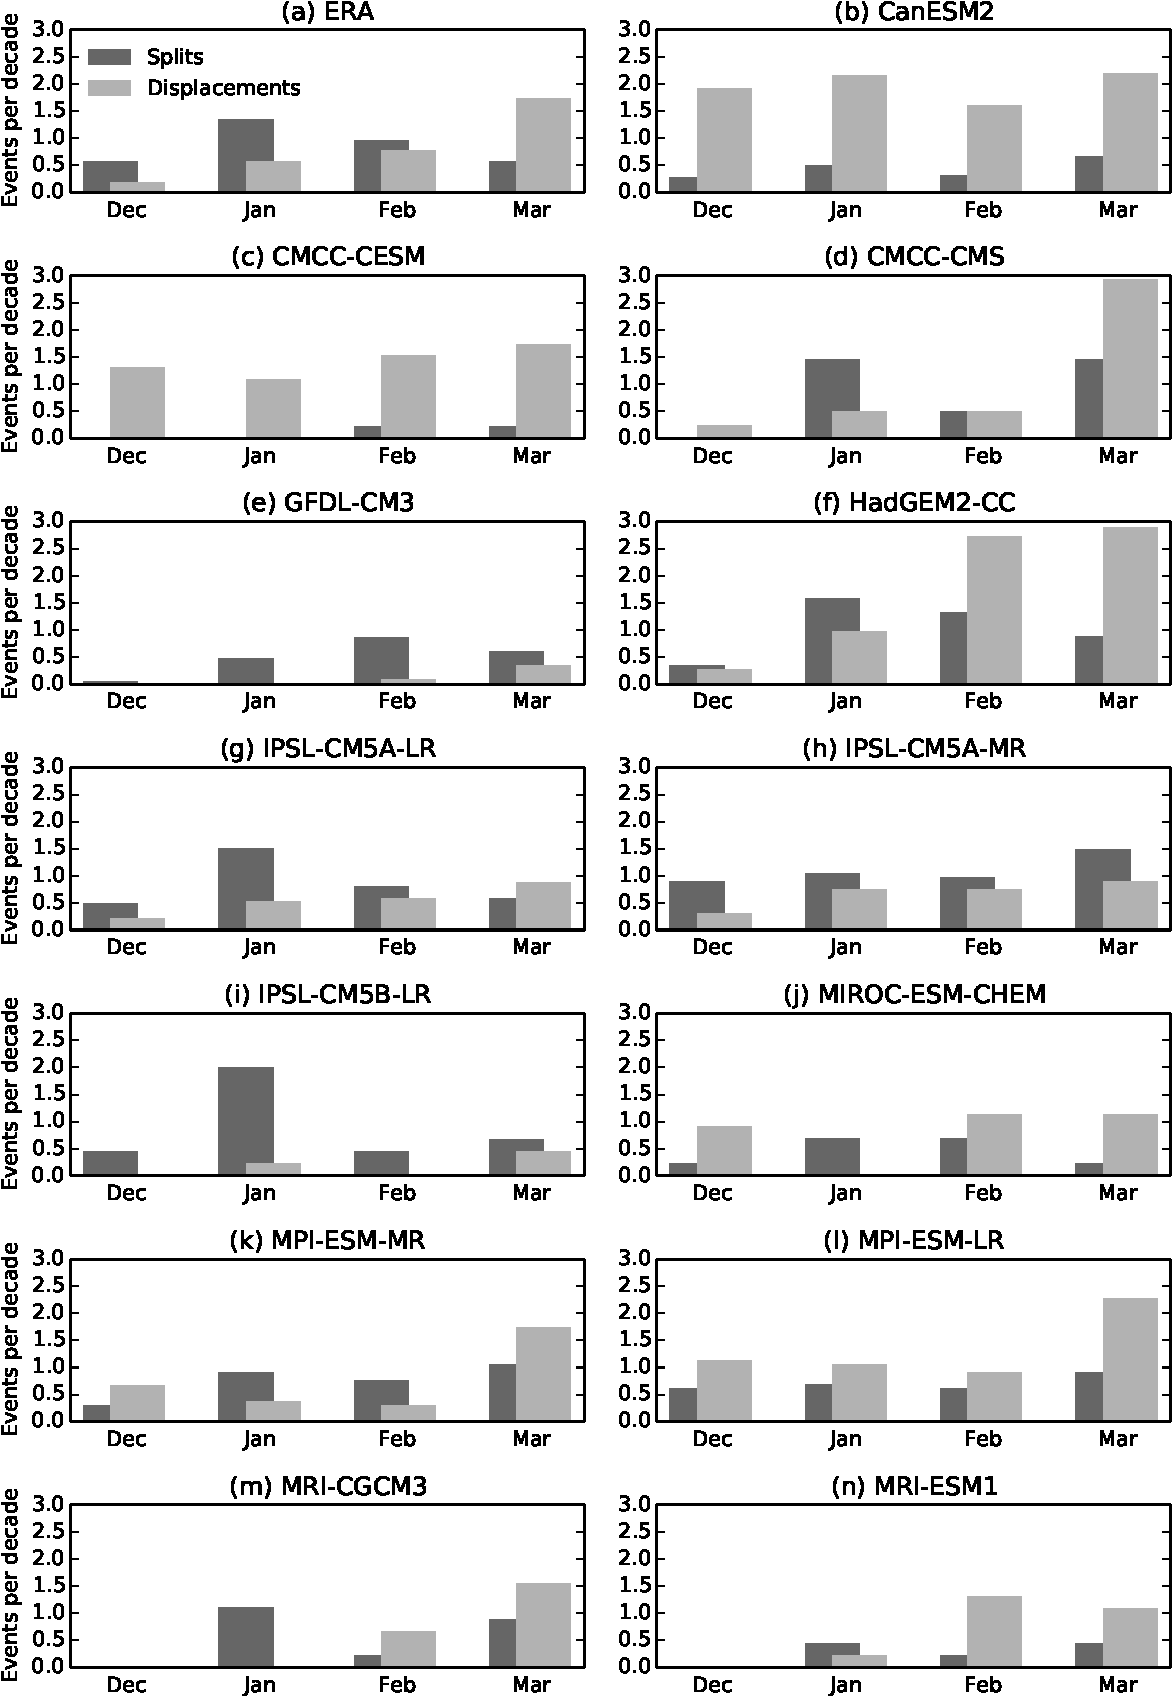
\includegraphics[width=\textwidth]{figures/chapter-models/events_seasonal.pdf}
 \caption[]{}
 \label{Fig2}
 \end{figure}



 \begin{figure}
 \centering
 \noindent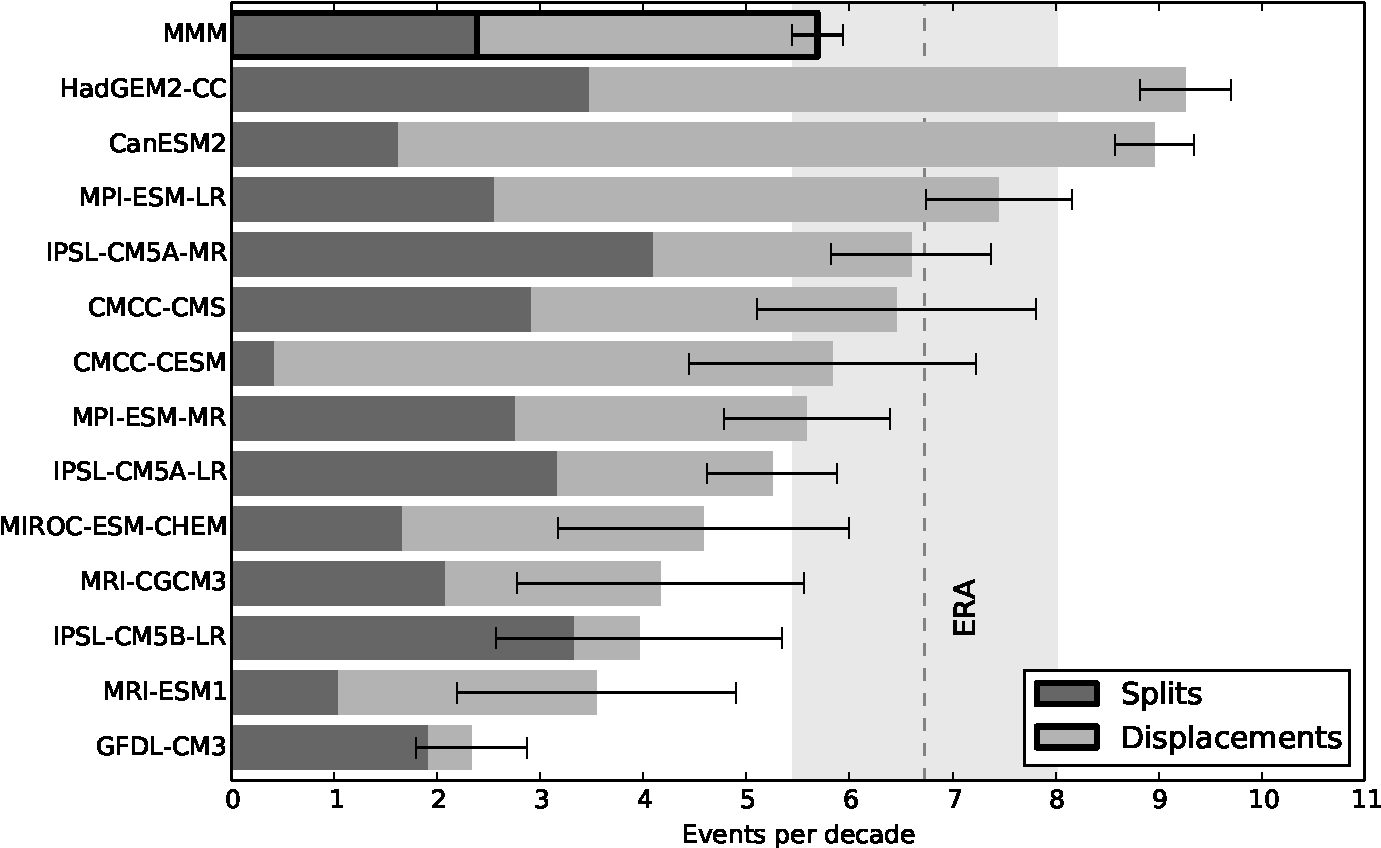
\includegraphics[width=\textwidth]{figures/chapter-models/events_bar_stacked.pdf}
 \caption[]{}
 \label{Fig2}
 \end{figure}



%%% Local Variables:
%%% mode: latex
%%% TeX-master: "thesis"
%%% End:
